\section{Experimentació}

\subsection{Se\lgem ecció dels operadors}
Per a realitzar l'experiment 1 ha fixat en nombre d'usuaris a 200 i el nombre de conductors a 100.
Posteriorment s'ha executat 10 cops amb cada un dels conjunts d'operadors.


Els resultats són ja donats les mitjes són:

\begin{center}
\begin{tabular}{l|cccc}
         & Temps & Conductors & Distància & Estats (aprox)\\
\hline
Conjunt 1 & 0:02:14 & 98 & 1009304 & 9950 \\
Conjunt 2 & 0:01:30 & 98 & 1113629 & 5200
\end{tabular}
\end{center}


\begin{figure}[H]
\begin{center}
 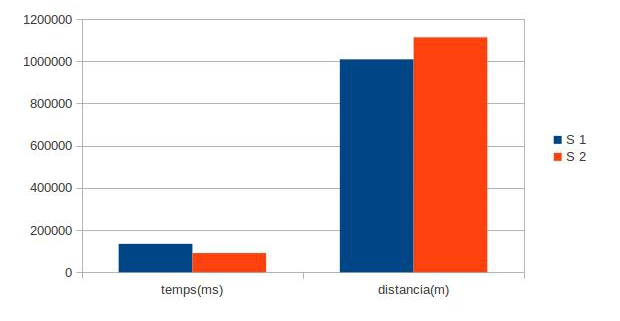
\includegraphics[width=0.6\textwidth]{figures/test1-gr1.jpg}
 \label{test1-gr1}
\caption{Test 1}
\end{center}
\end{figure}
                

El conjunt d'operadors 1 produeix millor resultat que el conjunt 2.
Suposam que això és degut a que l'operador genera mes estats (gairebé el doble) per a cada iteració i simplement a més estats per triar s'agafen més bons.

Es pot veure que el conjunt 2 es notablement més ràpid però no en la mateix proporció que els estats generats. Això es deu a que aquests estats
son més costosos, entre d'altres coses perquè un intercanvi implica dues operacions mentre que un canvi només una, entre d'altres detalls d'ambdós operadors.


\subsection{Se\lgem ecció de la generació de l'estat inicial}
Per realitzar l'experiment 2 s'ha fixat el nombre d'usuaris i el nombre de conductors com a l'anterior experiment.                                                                                   
S'ha executat 10 cops amb cada estratègia de generació inicial.
                                                                                                                                                                                                     
Els resultats són:


\begin{center}
\begin{tabular}{l|ccc}
         & Temps & Conductors & Distància\\
\hline
\emph{all one first} & 0:01:51 & 98 & 974543  \\
\emph{full first} & 0:02:08 & 98 & 1030151 
\end{tabular}
\end{center}

\begin{figure}[H]
\begin{center}
 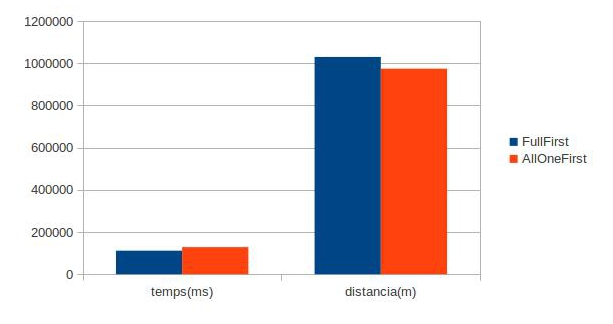
\includegraphics[width=0.6\textwidth]{figures/test2-gr1.jpg}
 \label{test2-gr1}
\caption{Test 2}
\end{center}
\end{figure}
                                                                                                                                                                                  
La estratègia de generació inicial \emph{all one first} produeix millors resultats tant en temps com distància,
aquest fet es deu a que te els passatgers més repartits en contraposició al \emph{full first} que els te
condensats i tarda més en repartir-los de manera adequada. De fet no te gaire sentit que els conductors
viatgin buits a l'inici ja que hem descartat el conjunt d'operadors que tal vegada haguessin pogut
jugar un bon paper amb el \emph{full first}.

\subsection{Se\lgem ecció dels paràmetres del Simulated Anealing}
Per a determinar els paràmetres que obtenen un millor resultat per a l'execució de l'algorisme \emph{simulated annealing},
hem executat reiterades vegades, aproximadament 10, l'algorisme amb diferents paràmetres per a $\lambda$ i \emph{k}, concretament s'ha fet amb
\texttt{[0.1,0.01,0.001,0.0001]} i \texttt{[1,5,25,125]} respectivament, fixant el nombre d'iteracions en 2000.

El millor resultat s'ha obtingut amb els paràmetres $k$ = 5 i $\lambda$ = 0.01, com indica el següent gràfic (fig. \ref{test3-gr1}).

\begin{figure}[H]
\begin{center} 
 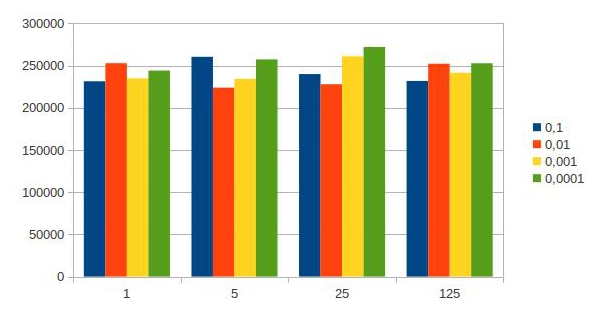
\includegraphics[width=0.6\textwidth]{figures/test3-gr1.jpg}
\label{test3-gr1}
\caption{Evolució de $\lambda$}
\end{center}
\end{figure}

Fixats aquests dos paràmetres en els valors que han obtingut millor resultat, s'ha ajustat el nombre d'iteracions executant diverses 
vegades l'algorisme amb un nombre diferent d'iteracions. Es pot veure (fig. \ref{test3-gr2}) en el següent gràfic el millor valor per al nombre d'iteracions.

\begin{figure}[H]
\begin{center}
 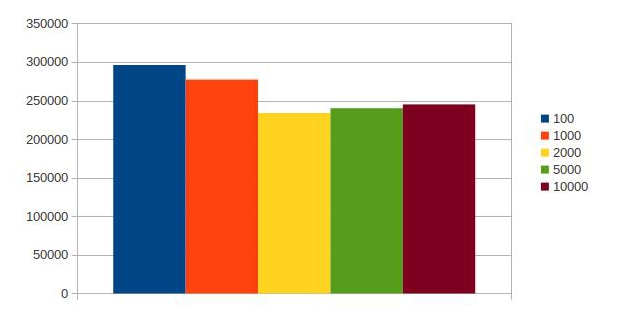
\includegraphics[width=0.6\textwidth]{figures/test3-gr2.jpg}
 \label{test3-gr2}
\caption{Evolució de \emph{k}}
\end{center}
\end{figure}


Aleshores, podem comparar els resultats obtinguts amb simulated Annealing i Hill climbing (fig. \ref{test3-gr3} i \ref{test3-gr4}).


\begin{figure}[H]
\begin{center} 
 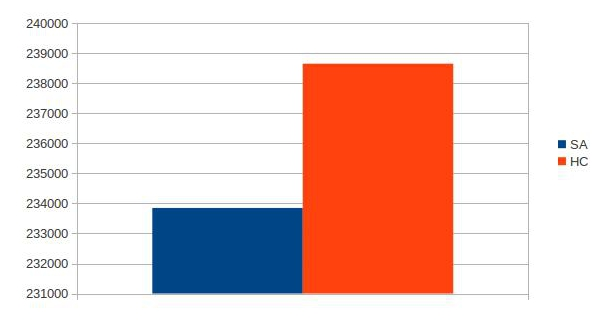
\includegraphics[width=0.6\textwidth]{figures/test3-gr3.jpg}
\label{test3-gr3}
\caption{}
\end{center}
\end{figure}


\begin{figure}[H]
\begin{center}
 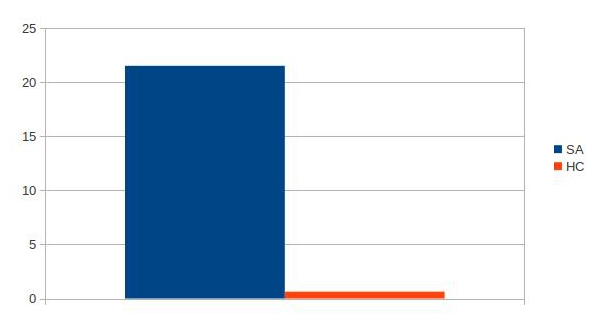
\includegraphics[width=0.6\textwidth]{figures/test3-gr4.jpg}
 \label{test3-gr4}
\caption{}
\end{center}
\end{figure}

Es pot observar que el Simulated Annealing obté millors resultats que el Hill Climbing. Per contra, té un temps d'execució molt més elevat.


\subsection{Observació de l'evolució temporal del Hill Climbing}
Per a l'experiment 4 s'ha fixat el nombre d'usuaris i el nombre de conductors com a l'experiment inicial.
En aquest cas, s'utilitza el conjunt d'operadors 1, i l'algorisme de generació d'estats inicials \emph{all one first}.
S'ha executat 10 vegades cada simulació.

Es pot observar com el temps d'execució segueix clarament un patró quadràtic ascendent en funció del nombre d'usuaris
del servei.

\begin{figure}[H]
\begin{center}
 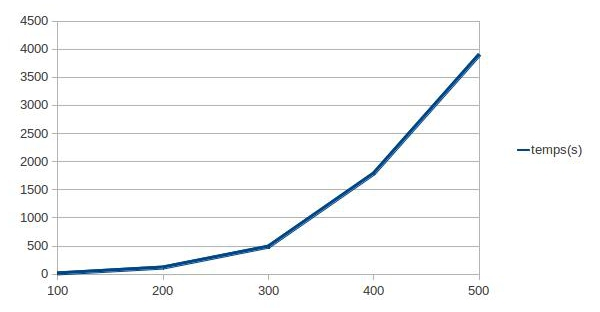
\includegraphics[width=0.6\textwidth]{figures/test4-gr1.jpg}
 \label{test4-gr1}
\caption{Evolució temporal en funció del nombre d'usuaris}
\end{center}
\end{figure}


\subsection{Comparació \emph{Hill Climbing} i \emph{Simulated Annealing} amb els dos heurístics}

\begin{center}
\begin{tabular}{l|llll}
 & \multicolumn{2}{c}{Hill Climbing} & \multicolumn{2}{c}{Simulated Annealing}\\
           & km       & veh       & km        & veh\\
\hline
temps      & 0:00:30  &  0:00:40  &  0:00:46  &  0:00:47\\
disntacia  & 549300   & 556103    &  857856   & 891356\\
conductors & 49       & 8         & 50        & 50\\
heurístic  & 549300   & 386556103 & 857856    & 500891356
\end{tabular}
\end{center}

\begin{figure}[H]
\begin{center}
 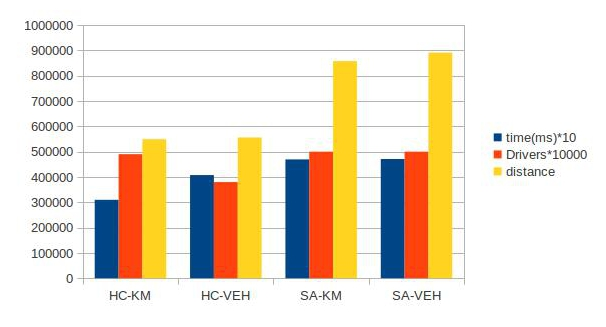
\includegraphics[width=0.6\textwidth]{figures/test6-gr1.jpg}
 \label{test6-gr1}
\caption{Compració HC vs SA}
\end{center}
\end{figure}

D'aquests resultats observam que l'algorisme \emph{Hill Climbing} troba millors solucions que el \emph{Simulated Annealing} si disposa d'un temps similar.
Suposam que augmentant el nombre d'iteracions del \emph{Simulated Annealing} podríem aconseguir millors resultats que amb el \emph{Hill climbing}.


S'observa també que els dos heurístics funcionen com esperàvem en el cas de \emph{Hill Climbing},(disminuint el nombre de km en un cas
i el nombre de km i conductors en l'altre), però en el \emph{Simulated Annealing} s'obté un resultat similar.
Es possible que això sigui degut a que els heurístics s'han ponderat utilitzat \emph{Hill Climbing}.

En aquest experiment sembla que ens decantaríem en favor de \emph{Hill Climbing}.






\subsection{Se\lgem ecció del valor de \emph{M} per millor inicialització del problema}
Per a realitzar l'experiment 7 s'ha se\lgem eccionat un problema de mida 50 usuaris, i s'ha provat per a totes les proporcions
(de tots conductors fins a un sol conductor), 10 cops cada una.

Es pot observar al següent gràfic que les so\lgem ucions més benevolents s'obtenen aproximadament per a 30 conductors (20 no conductors al gràfic),
que podem extrapolar aproximadament $\dfrac{3}{5}$ de conductors del total per a qualsevol problema.
Els valors en que no s'ha trobat so\lgem ució (a partir de 34) no es mostren.

\begin{figure}[H]
\begin{center}
 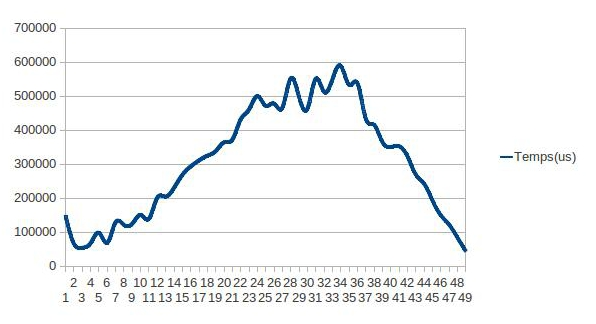
\includegraphics[width=0.6\textwidth]{figures/test7-gr1.jpg}
 \label{test7-gr2}
\end{center}
\caption{Evolució del la distància}
\end{figure}

Per al temps de trobar una so\lgem ució, podem observar que on més temps es tarda es a una proporció de $\dfrac{2}{5}$ conductors.
Intuïm que es la zona on es generen mes intercanvis de passatgers, ja que n'hi ha suficients per a generar molts d'estats,
però no massa com per a que molts d'estats no siguin vàlids.
Amb una proporció més alta de passatgers es triga menys temps, però com hem explicat anteriorment es difícil trobar una so\lgem ució que satisfaci les restriccions.

\begin{figure}[H]
\begin{center}
 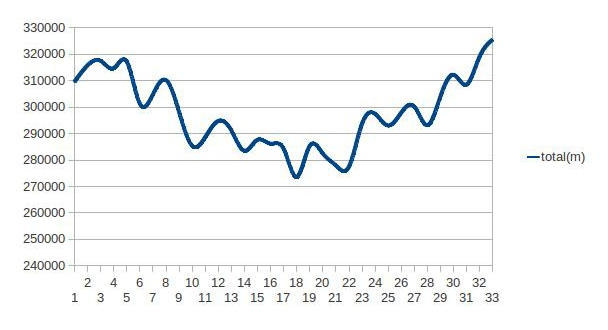
\includegraphics[width=0.6\textwidth]{figures/test7-gr2.jpg}
 \label{test7-gr2}
\end{center}
\caption{Evolució del temps}
\end{figure}
        
